\section{Scale dependent systematics}\label{sec:scalesys}
\mr{HERE} We further test the stability of our results by extending the highest mode from $\ell=20$ to $100$, or fluctuations over scales as small as $1.8$ degrees (see, Fig. \ref{fig:chi2cellextend}). The solid line shows how the median of 1000 mocks changes as the highest $\ell$ increases from $20$ to $100$. The red circles show the chi2 for the linear approach with three maps and the blue crosses show the chi2 for the nonlinear approach with three maps. \mr{However, as we show later, our second diagnostic based on the mean density contrast reveals that there is a residual systematic error against the z-band depth with the linear cleaning approach even though the z-band depth was an input for training. }

\begin{figure}
\centering
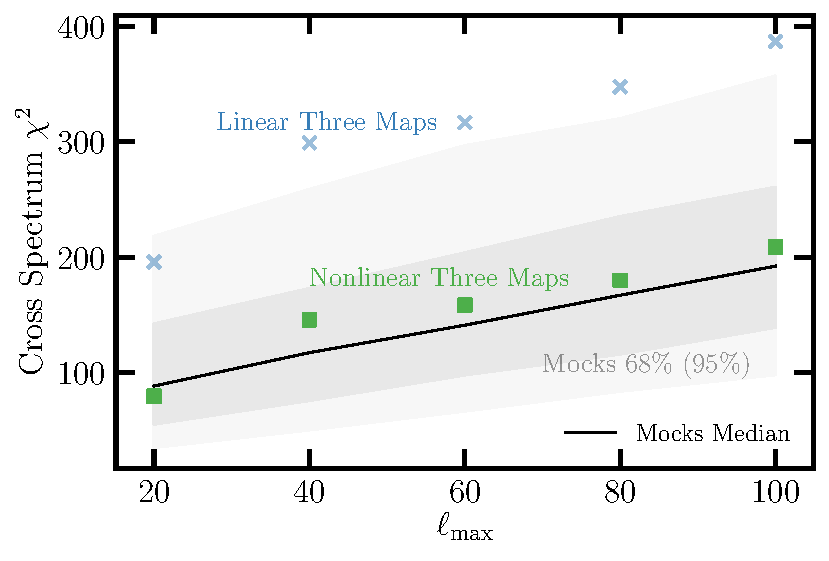
\includegraphics[width=0.5\textwidth]{chi2lmax.pdf}
\caption{Cross power spectrum $\chi^{2}$ as a function of the highest mode $\ell_{\rm max}$ for the DR9 LRG sample using the linear and nonlinear imaging weights with the conservative II maps. The lowest mode is fixed at $\ell_{\rm min}=2$. Solid curve and dark (light) shade represent the median estimate and $68\%$ ($95\%$) confidence constructed from the $\fnl=0$ mocks.}\label{fig:chi2cellextend}
\end{figure}


%\section{Redshift distribution}
%Redshift distribution of LRGs is constructed from the DESI SV data release of Denali with the same selection. The fiducial distribution only covers the redshift range from 0.2 to 1.35. Below we test the impact of LRG dN/dz on the angular power spectrum.
%
%
%\begin{figure}
%\centering
%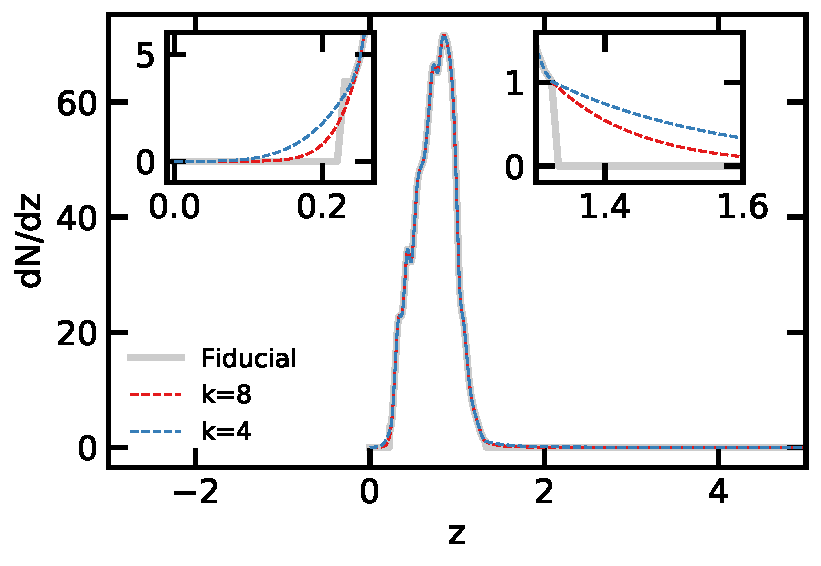
\includegraphics[width=0.45\textwidth]{nztreat.pdf}
%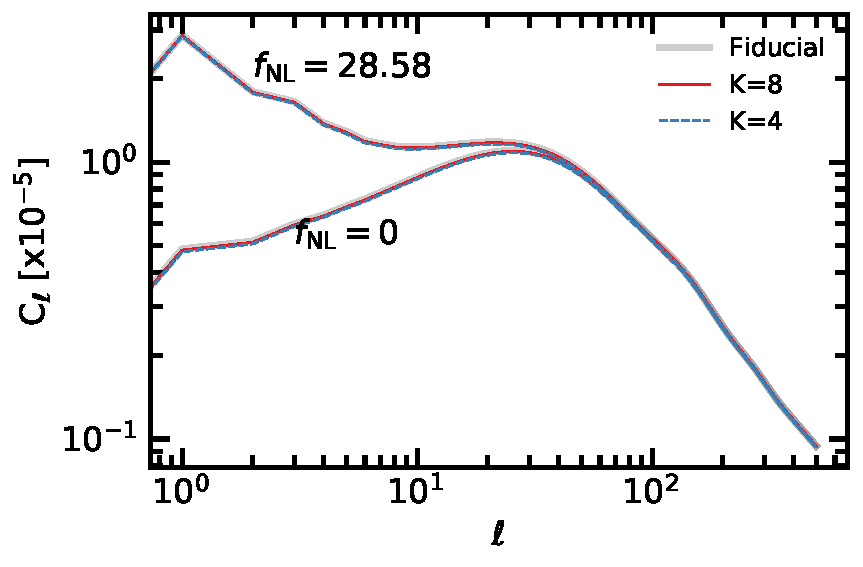
\includegraphics[width=0.45\textwidth]{cell_nz.pdf}
%\caption{Top: Redshift distribution of LRGs. Bottom: Power spectrum given various dN/dz treatments for two arbitrary $\fnl$ values.}
%\end{figure}